\documentclass{article}
\usepackage[12pt]{extsizes}
\usepackage{cmap}
\usepackage[utf8]{inputenc}
%\usepackage[cp1251]{inputenc}
\usepackage[T2A]{fontenc}
\usepackage[russian]{babel}
\usepackage{color}
\usepackage{hyperref}
\usepackage{enumerate}
\usepackage{amsmath,amssymb, wasysym}
\numberwithin{equation}{section}
\makeatletter
\@addtoreset{equation}{section}
\makeatother
%\usepackage{chngcntr}
%\counterwithin{equation}{section}
\usepackage{enumitem}
\usepackage{epstopdf}
\usepackage{graphicx}
\usepackage[warn]{mathtext} 

%\graphicspath{{noiseimages/}}
\hypersetup{unicode = true, colorlinks, citecolor = red, filecolor = red, linkcolor = blue, urlcolor = blue }

\usepackage[left=2cm,right=2cm,
    top=2cm,bottom=2cm,bindingoffset=0cm]{geometry}
    
    \RequirePackage{caption2} 
\renewcommand\captionlabeldelim{ -} 

\begin{document}

\def\figurename{Рисунок}



\pagestyle{empty}
\begin{center}

{\LARGE\bf{Мануал. Программа NeiSys}}\par
\Large{Трофимов Е.П.}

\end{center}

 %\par \par *Конспект написан с целью 
\newpage



\setcounter{tocdepth}{2}  %numiric of pages
\tableofcontents


\newpage




%%%%%%%%%%%%%%%%%%%%%%%%%%%%%%%%%%%%%%%%%%%%%%%%%%%%%%%%%%%%%%%%%%%%%%%%%%%%%%%%%%%%%%%%%%%%%%%%%%%%%%%%%%%%%%%%%%%%%%%%%%%%%%%%%%%%%%%
\section{Практическое руководство}
%%%%%%%%%%%%%%%%%%%%%%%%%%%%%%%%%%%%%%%%%%%%%%%%%%%%%%%%%%%%%%%%%%%%%%%%%%%%%%%%%%%%%%%%%%%%%%%%%%%%%%%%%%%%%%%%%%%%%%%%%%%%%%%%%%%%%%%
\subsection{Запуск}


\qquad Для установки необходимо установить JVM (Java Virtual Mashine). Для этого заходим на \href{https://java.com/ru/download/manual.jsp}{официальный сайт Java}, скачиваем версию, соотвутствующую нашей операционной системе, устанавливаем и перезагружаем компьютер. 

После этого можно запускать программу - открываем файл {\bf NeiSys.jar}. После запуска должно появиться следующее окно:

\begin{figure}[h]
\center{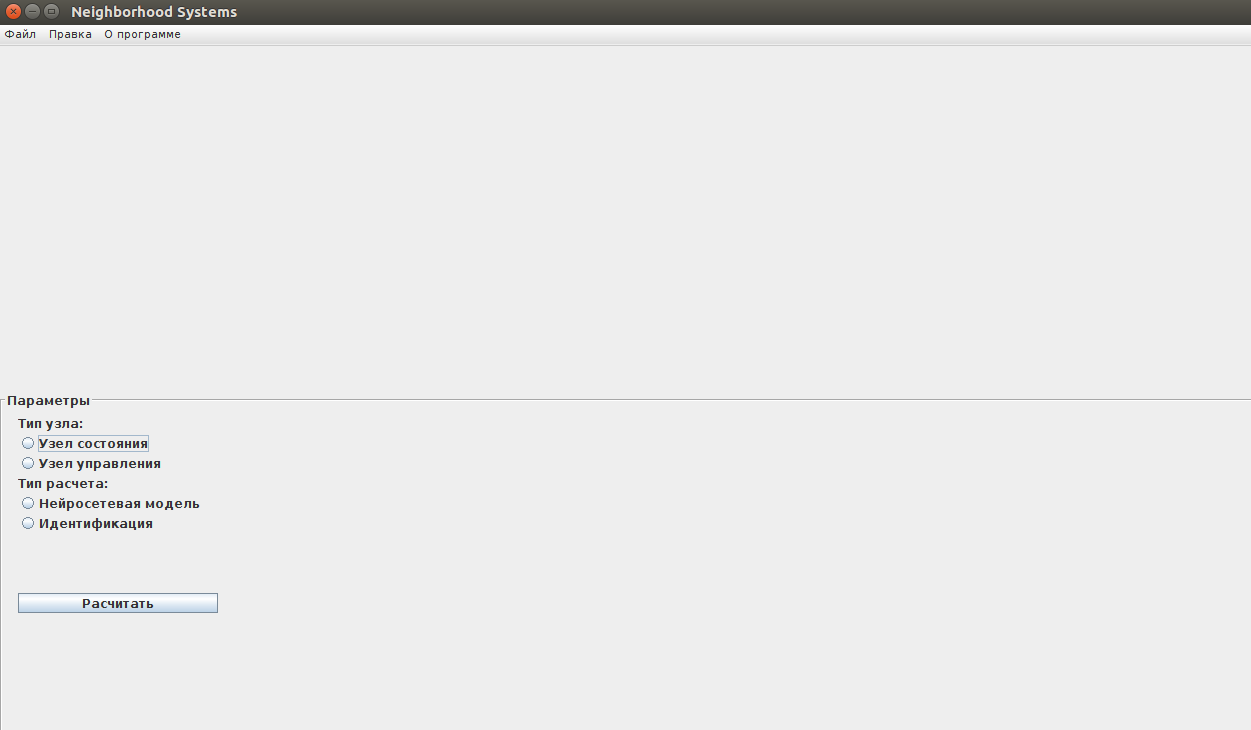
\includegraphics[width=0.8\linewidth]{pic/start.png}}
\caption{Стартовая панель программы.}
\label{ris:image}
\end{figure}

Если же данное окно не появилось, вероятнее всего что-то пошло не так при установке Java. Проверьте еще, правильно ли прошла установка. Возможно понадобиться прописать переменную JAVA\_HOME (возможные ошибки при установке Java не такая уж редкость, поэтому решение большинства из них можно прогуглить, например, \href{https://www.java.com/ru/download/help/path.xml}{настройка системной переменной}).

\subsection{Описание простейшего функционала}


\subsection{Вычисения}


\newpage

\section{Руководство для программистов}

\subsection{Структура программы}
UML-диграмма:

\begin{figure}[h]
\center{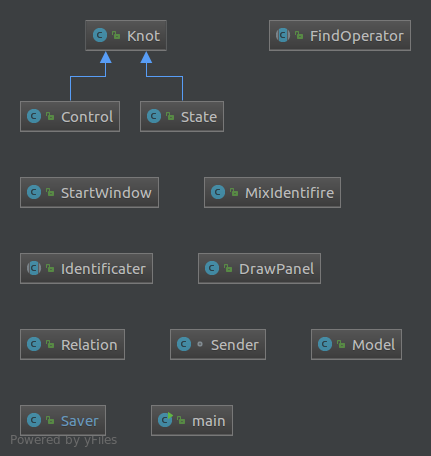
\includegraphics[width=0.3\linewidth]{pic/umlDiag.png}}
\caption{UML-диаграмма.}
\label{ris:image}
\end{figure}



\end{document}
\grid
\grid
\grid
\grid
